% Generated by Sphinx.
\def\sphinxdocclass{report}
\documentclass[letterpaper,10pt,english]{sphinxmanual}
\usepackage[utf8]{inputenc}
\DeclareUnicodeCharacter{00A0}{\nobreakspace}
\usepackage[T1]{fontenc}
\usepackage{babel}
\usepackage{times}
\usepackage[Bjarne]{fncychap}
\usepackage{longtable}
\usepackage{sphinx}
\usepackage{multirow}


\title{PyRE Documentation}
\date{May 11, 2013}
\release{5.0.1}
\author{Juergen Hackl}
\newcommand{\sphinxlogo}{}
\renewcommand{\releasename}{Release}
\makeindex

\makeatletter
\def\PYG@reset{\let\PYG@it=\relax \let\PYG@bf=\relax%
    \let\PYG@ul=\relax \let\PYG@tc=\relax%
    \let\PYG@bc=\relax \let\PYG@ff=\relax}
\def\PYG@tok#1{\csname PYG@tok@#1\endcsname}
\def\PYG@toks#1+{\ifx\relax#1\empty\else%
    \PYG@tok{#1}\expandafter\PYG@toks\fi}
\def\PYG@do#1{\PYG@bc{\PYG@tc{\PYG@ul{%
    \PYG@it{\PYG@bf{\PYG@ff{#1}}}}}}}
\def\PYG#1#2{\PYG@reset\PYG@toks#1+\relax+\PYG@do{#2}}

\def\PYG@tok@gd{\def\PYG@tc##1{\textcolor[rgb]{0.63,0.00,0.00}{##1}}}
\def\PYG@tok@gu{\let\PYG@bf=\textbf\def\PYG@tc##1{\textcolor[rgb]{0.50,0.00,0.50}{##1}}}
\def\PYG@tok@gt{\def\PYG@tc##1{\textcolor[rgb]{0.00,0.25,0.82}{##1}}}
\def\PYG@tok@gs{\let\PYG@bf=\textbf}
\def\PYG@tok@gr{\def\PYG@tc##1{\textcolor[rgb]{1.00,0.00,0.00}{##1}}}
\def\PYG@tok@cm{\let\PYG@it=\textit\def\PYG@tc##1{\textcolor[rgb]{0.25,0.50,0.56}{##1}}}
\def\PYG@tok@vg{\def\PYG@tc##1{\textcolor[rgb]{0.73,0.38,0.84}{##1}}}
\def\PYG@tok@m{\def\PYG@tc##1{\textcolor[rgb]{0.13,0.50,0.31}{##1}}}
\def\PYG@tok@mh{\def\PYG@tc##1{\textcolor[rgb]{0.13,0.50,0.31}{##1}}}
\def\PYG@tok@cs{\def\PYG@tc##1{\textcolor[rgb]{0.25,0.50,0.56}{##1}}\def\PYG@bc##1{\colorbox[rgb]{1.00,0.94,0.94}{##1}}}
\def\PYG@tok@ge{\let\PYG@it=\textit}
\def\PYG@tok@vc{\def\PYG@tc##1{\textcolor[rgb]{0.73,0.38,0.84}{##1}}}
\def\PYG@tok@il{\def\PYG@tc##1{\textcolor[rgb]{0.13,0.50,0.31}{##1}}}
\def\PYG@tok@go{\def\PYG@tc##1{\textcolor[rgb]{0.19,0.19,0.19}{##1}}}
\def\PYG@tok@cp{\def\PYG@tc##1{\textcolor[rgb]{0.00,0.44,0.13}{##1}}}
\def\PYG@tok@gi{\def\PYG@tc##1{\textcolor[rgb]{0.00,0.63,0.00}{##1}}}
\def\PYG@tok@gh{\let\PYG@bf=\textbf\def\PYG@tc##1{\textcolor[rgb]{0.00,0.00,0.50}{##1}}}
\def\PYG@tok@ni{\let\PYG@bf=\textbf\def\PYG@tc##1{\textcolor[rgb]{0.84,0.33,0.22}{##1}}}
\def\PYG@tok@nl{\let\PYG@bf=\textbf\def\PYG@tc##1{\textcolor[rgb]{0.00,0.13,0.44}{##1}}}
\def\PYG@tok@nn{\let\PYG@bf=\textbf\def\PYG@tc##1{\textcolor[rgb]{0.05,0.52,0.71}{##1}}}
\def\PYG@tok@no{\def\PYG@tc##1{\textcolor[rgb]{0.38,0.68,0.84}{##1}}}
\def\PYG@tok@na{\def\PYG@tc##1{\textcolor[rgb]{0.25,0.44,0.63}{##1}}}
\def\PYG@tok@nb{\def\PYG@tc##1{\textcolor[rgb]{0.00,0.44,0.13}{##1}}}
\def\PYG@tok@nc{\let\PYG@bf=\textbf\def\PYG@tc##1{\textcolor[rgb]{0.05,0.52,0.71}{##1}}}
\def\PYG@tok@nd{\let\PYG@bf=\textbf\def\PYG@tc##1{\textcolor[rgb]{0.33,0.33,0.33}{##1}}}
\def\PYG@tok@ne{\def\PYG@tc##1{\textcolor[rgb]{0.00,0.44,0.13}{##1}}}
\def\PYG@tok@nf{\def\PYG@tc##1{\textcolor[rgb]{0.02,0.16,0.49}{##1}}}
\def\PYG@tok@si{\let\PYG@it=\textit\def\PYG@tc##1{\textcolor[rgb]{0.44,0.63,0.82}{##1}}}
\def\PYG@tok@s2{\def\PYG@tc##1{\textcolor[rgb]{0.25,0.44,0.63}{##1}}}
\def\PYG@tok@vi{\def\PYG@tc##1{\textcolor[rgb]{0.73,0.38,0.84}{##1}}}
\def\PYG@tok@nt{\let\PYG@bf=\textbf\def\PYG@tc##1{\textcolor[rgb]{0.02,0.16,0.45}{##1}}}
\def\PYG@tok@nv{\def\PYG@tc##1{\textcolor[rgb]{0.73,0.38,0.84}{##1}}}
\def\PYG@tok@s1{\def\PYG@tc##1{\textcolor[rgb]{0.25,0.44,0.63}{##1}}}
\def\PYG@tok@gp{\let\PYG@bf=\textbf\def\PYG@tc##1{\textcolor[rgb]{0.78,0.36,0.04}{##1}}}
\def\PYG@tok@sh{\def\PYG@tc##1{\textcolor[rgb]{0.25,0.44,0.63}{##1}}}
\def\PYG@tok@ow{\let\PYG@bf=\textbf\def\PYG@tc##1{\textcolor[rgb]{0.00,0.44,0.13}{##1}}}
\def\PYG@tok@sx{\def\PYG@tc##1{\textcolor[rgb]{0.78,0.36,0.04}{##1}}}
\def\PYG@tok@bp{\def\PYG@tc##1{\textcolor[rgb]{0.00,0.44,0.13}{##1}}}
\def\PYG@tok@c1{\let\PYG@it=\textit\def\PYG@tc##1{\textcolor[rgb]{0.25,0.50,0.56}{##1}}}
\def\PYG@tok@kc{\let\PYG@bf=\textbf\def\PYG@tc##1{\textcolor[rgb]{0.00,0.44,0.13}{##1}}}
\def\PYG@tok@c{\let\PYG@it=\textit\def\PYG@tc##1{\textcolor[rgb]{0.25,0.50,0.56}{##1}}}
\def\PYG@tok@mf{\def\PYG@tc##1{\textcolor[rgb]{0.13,0.50,0.31}{##1}}}
\def\PYG@tok@err{\def\PYG@bc##1{\fcolorbox[rgb]{1.00,0.00,0.00}{1,1,1}{##1}}}
\def\PYG@tok@kd{\let\PYG@bf=\textbf\def\PYG@tc##1{\textcolor[rgb]{0.00,0.44,0.13}{##1}}}
\def\PYG@tok@ss{\def\PYG@tc##1{\textcolor[rgb]{0.32,0.47,0.09}{##1}}}
\def\PYG@tok@sr{\def\PYG@tc##1{\textcolor[rgb]{0.14,0.33,0.53}{##1}}}
\def\PYG@tok@mo{\def\PYG@tc##1{\textcolor[rgb]{0.13,0.50,0.31}{##1}}}
\def\PYG@tok@mi{\def\PYG@tc##1{\textcolor[rgb]{0.13,0.50,0.31}{##1}}}
\def\PYG@tok@kn{\let\PYG@bf=\textbf\def\PYG@tc##1{\textcolor[rgb]{0.00,0.44,0.13}{##1}}}
\def\PYG@tok@o{\def\PYG@tc##1{\textcolor[rgb]{0.40,0.40,0.40}{##1}}}
\def\PYG@tok@kr{\let\PYG@bf=\textbf\def\PYG@tc##1{\textcolor[rgb]{0.00,0.44,0.13}{##1}}}
\def\PYG@tok@s{\def\PYG@tc##1{\textcolor[rgb]{0.25,0.44,0.63}{##1}}}
\def\PYG@tok@kp{\def\PYG@tc##1{\textcolor[rgb]{0.00,0.44,0.13}{##1}}}
\def\PYG@tok@w{\def\PYG@tc##1{\textcolor[rgb]{0.73,0.73,0.73}{##1}}}
\def\PYG@tok@kt{\def\PYG@tc##1{\textcolor[rgb]{0.56,0.13,0.00}{##1}}}
\def\PYG@tok@sc{\def\PYG@tc##1{\textcolor[rgb]{0.25,0.44,0.63}{##1}}}
\def\PYG@tok@sb{\def\PYG@tc##1{\textcolor[rgb]{0.25,0.44,0.63}{##1}}}
\def\PYG@tok@k{\let\PYG@bf=\textbf\def\PYG@tc##1{\textcolor[rgb]{0.00,0.44,0.13}{##1}}}
\def\PYG@tok@se{\let\PYG@bf=\textbf\def\PYG@tc##1{\textcolor[rgb]{0.25,0.44,0.63}{##1}}}
\def\PYG@tok@sd{\let\PYG@it=\textit\def\PYG@tc##1{\textcolor[rgb]{0.25,0.44,0.63}{##1}}}

\def\PYGZbs{\char`\\}
\def\PYGZus{\char`\_}
\def\PYGZob{\char`\{}
\def\PYGZcb{\char`\}}
\def\PYGZca{\char`\^}
\def\PYGZsh{\char`\#}
\def\PYGZpc{\char`\%}
\def\PYGZdl{\char`\$}
\def\PYGZti{\char`\~}
% for compatibility with earlier versions
\def\PYGZat{@}
\def\PYGZlb{[}
\def\PYGZrb{]}
\makeatother

\begin{document}

\maketitle
\tableofcontents
\phantomsection\label{index::doc}


Contents:


\chapter{Introduction}
\label{README:introduction}\label{README:pyre-documentation}\label{README::doc}\begin{quote}\begin{description}
\item[{Date}] \leavevmode
11 May 2013

\item[{Authors}] \leavevmode
Jürgen Hackl

\item[{Contact}] \leavevmode
\href{mailto:hackl.j@gmx.at}{hackl.j@gmx.at}

\item[{Web site}] \leavevmode
\href{http://github.com/hackl/pyre}{http://github.com/hackl/pyre}

\item[{Copyright}] \leavevmode
This document has been placed in the public domain.

\item[{License}] \leavevmode
PyRe is released under the GNU General Public Licence.

\item[{Version}] \leavevmode
5.0.1

\end{description}\end{quote}

\begin{notice}{warning}{Warning:}
This is a preliminary program code!

I wrote \code{pyre} for my Master's Thesis.
The work isn't finished yet, so changes in the code are very likely!
\end{notice}

\begin{notice}{note}{Note:}
If you have any problems, found bugs in the code or have feature request
comments or questions, please feel free to send a mail to \href{mailto:hackl.j@gmx.at}{Jürgen Hackl}.
\end{notice}


\section{Purpose}
\label{README:jurgen-hackl}\label{README:purpose}
PyRe (python Reliability) is a python module for structural reliability
analysis. Its flexibility and extensibility make it applicable to a large
suite of problems. Along with core reliability analysis functionality, PyRe
includes methods for summarizing output.

\begin{notice}{note}{Note:}
At the moment only First-Order Reliability Methods are supported!
Second-Order Reliability Methods and Monte Carlo Simulation will hopefully
follow soon :)
\end{notice}


\section{History}
\label{README:history}
The FERUM (Finite Element Reliability Using Matlab) project was initiated in
1999 at the University of California, Berkeley, by Terje Haukaas and Armen Der
Kiureghian, primarily for pedagogical purposes aimed at teaching and learning
structural reliability and stochastic finite elements methods. {\hyperref[references:derkiureghian2006]{{[}DerKiureghian2006{]}}}
This code consists of an open-source Matlab toolbox, featuring various
structural reliability methods. The latest available version (version 3.1),
which can be downloaded from \href{http://www.ce.berkeley.edu/projects/ferum/}{FERUM}. Since 2003, this code is no longer
officially maintained. {\hyperref[references:bourinet2010]{{[}Bourinet2010{]}}}

A new version of this open-source code (FERUM 4.x) based on a work carried out
at the Institut Français de Mécanique Avancée (\href{http://www.ifma.fr/Recherche/Labos/FERUM}{IFMA}) in Clermont-Ferrand,
France. This version offers improved capabilities such as simulation-based
technique (Subset Simulation), Global Sensitivity Analysis (based on Sobol’s
indices), Reliability-Based Design Optimization (RBDO) algorithm, Global
Sensitivity Analysis and reliability assessment based on Support Vector
Machine (SVM) surrogates, etc. Beyond the new methods implemented in this
Matlab code. {\hyperref[references:bourinet2009]{{[}Bourinet2009{]}}}

Of the purpose, to use structural reliability analysis for the project ``Risk
based decision framework for the optimal management of aging reinforced
concrete structures'' {\hyperref[references:hackl2013]{{[}Hackl2013{]}}} a python version of FERUM has been created.

The focus here lies on the reliability analysis and not more on the finite
element method, so only the core function of FERUM are implemented.


\section{Features}
\label{README:features}
PyRe provides functionalities to make structural reliability analysis as easy
as possible. Here is a short list of some of its features:
\begin{itemize}
\item {} 
Perform reliability analysis with First-Order Reliability Methods

\item {} 
Includes a large suite of well-documented statistical distributions.

\item {} 
Uses NumPy for numerics wherever possible.

\item {} 
No limitation on the limit state function

\item {} 
Correlation between the random variables are possible

\item {} 
Traces can be saved to the disk as plain text.

\item {} 
PyRe can be embedded in larger programs, and results can be analyzed
with the full power of Python.

\end{itemize}


\section{Getting started}
\label{README:getting-started}
This guide provides all the information needed to install PyRe, code a
reliability model, run the sampler, save and visualize the results. In
addition, it contains a list of the statistical distributions currently
available.


\chapter{Installation}
\label{install:installation}\label{install:ifma}\label{install::doc}\begin{quote}\begin{description}
\item[{Date}] \leavevmode
11 May 2013

\item[{Authors}] \leavevmode
Jürgen Hackl

\item[{Contact}] \leavevmode
\href{mailto:hackl.j@gmx.at}{hackl.j@gmx.at}

\item[{Web site}] \leavevmode
\href{http://github.com/hackl/pyre}{http://github.com/hackl/pyre}

\item[{Copyright}] \leavevmode
This document has been placed in the public domain.

\item[{License}] \leavevmode
PyRe is released under the GNU General Public Licence.

\item[{Version}] \leavevmode
5.0.1

\end{description}\end{quote}

PyRe is known to run on Mac OS X, Linux and Windows, but in theory should be
able to work on just about any platform for which Python, a Fortran compiler
and the NumPy SciPy, and Math modules are available. However, installing some
extra depencies can greatly improve PyRe's performance and versatility. The
following describes the required and optional dependencies and takes you
through the installation process.


\section{Dependencies}
\label{install:dependencies}
PyMC requires some prerequisite packages to be present on the system.
Fortunately, there are currently only a few hard dependencies, and all are
freely available online.
\begin{itemize}
\item {} 
\href{http://www.python.org/.}{Python} version 2.6 or later.

\item {} 
\href{http://www.scipy.org/NumPy}{NumPy} : The fundamental scientific programming package, it
provides a multidimensional array type and many useful functions for
numerical analysis.

\item {} 
\href{http://www.scipy.org/}{SciPy} : Library of algorithms for mathematics, science and engineering.

\item {} 
\href{http://ipython.scipy.org/}{IPython} (optional): An enhanced interactive Python shell and an
architecture for interactive parallel computing.

\end{itemize}


\section{Installation using EasyInstall}
\label{install:ipython}\label{install:installation-using-easyinstall}
Not available at the moment.


\section{Installing from pre-built binaries}
\label{install:installing-from-pre-built-binaries}
Not available at the moment.


\section{Compiling the source code}
\label{install:compiling-the-source-code}
First download the source code from \href{https://github.com/hackl/pyre}{GitHub} and unpack it. Then move
into the unpacked directory and follow the platform specific instructions.


\subsection{Windows}
\label{install:windows}
Not available at the moment.


\subsection{Mac OS X or Linux}
\label{install:mac-os-x-or-linux}
Not available at the moment.


\section{Development version}
\label{install:development-version}
You can check out the development version of the code from the \href{https://github.com/hackl/pyre}{GitHub}
repository:

\begin{Verbatim}[commandchars=\\\{\}]
git clone git://github.com/hackl/pyre.git
\end{Verbatim}


\section{Bugs and feature requests}
\label{install:github}\label{install:bugs-and-feature-requests}
Report problems with the installation, bugs in the code or feature request at
the \href{http://github.com/hackl/pyre/issues}{issue tracker}. Comments and questions are welcome and should be
addressed to \href{mailto:hackl.j@gmx.at}{Jürgen Hackl}.


\chapter{Tutorial}
\label{tutorial:chap-tutorial}\label{tutorial::doc}\label{tutorial:jurgen-hackl}\label{tutorial:tutorial}
This tutorial will guide you through a typical PyMC application. Familiarity
with Python is assumed, so if you are new to Python, books such as {\hyperref[references:lutz2007]{{[}Lutz2007{]}}}
or {\hyperref[references:langtangen2009]{{[}Langtangen2009{]}}} are the place to start. Plenty of online documentation
can also be found on the \href{http://www.python.org/doc/}{Python documentation} page.


\section{An example reliability model}
\label{tutorial:an-example-reliability-model}
Consider the following random variables:
\phantomsection\label{tutorial:equation-random_variables}
        \begin{align}
        X_1 &\sim \text{Logormal}(500,100)\\
        X_2 &\sim \text{Normal}(2000,400)\\
        X_3 &\sim \text{Uniform}(5,0.5)
        \end{align}

\label{tutorial-random_variables}

Additionaly those variables are relatet to each other. Therefore the
correlationmatrix ${\bf C}$ is given:
\phantomsection\label{tutorial:equation-correlation_matrix}\begin{gather}
\begin{split}        \begin{align}
        {\bf C} =
        \begin{pmatrix}
        1.0 & 0.3 & 0.2\\
        0.3 & 1.0 & 0.2\\
        0.2 & 0.2 & 1.0
        \end{pmatrix}
        \end{align}\end{split}\label{tutorial-correlation_matrix}
\end{gather}
Now, we like to compute the reliability index $\beta$ and the failure
probability $P_f$, by given limit state function $g(X_1,X_2,X_3)$:
\phantomsection\label{tutorial:equation-limit_state_function}\begin{gather}
\begin{split}        g(X_1,X_2,X_3) = 1 - \frac{X_2}{1000 \cdot X_3} -
        \left( \frac{X_1}{200 \cdot X_3} \right)^2\end{split}\label{tutorial-limit_state_function}
\end{gather}

\section{Let's model}
\label{tutorial:let-s-model}
Before we start with the modeling, we have to import the \code{pyre}
package. Therefore are two different methods available:

In case 1 we load \code{pyre} like a normal library:

\begin{Verbatim}[commandchars=\\\{\}]
\PYG{k+kn}{import} \PYG{n+nn}{pyre}
\end{Verbatim}

here we must write for each command \code{pyre.my\_command()}. A much nicer way to
load the package is case 2:

\begin{Verbatim}[commandchars=\\\{\}]
\PYG{c}{\PYGZsh{} import pyre library}
\PYG{k+kn}{from} \PYG{n+nn}{pyre} \PYG{k+kn}{import} \PYG{o}{*}
\end{Verbatim}

here, we import all available objects from \code{pyre}.

To define the random variables from \eqref{tutorial-random_variables} we can use
following syntax:

\begin{Verbatim}[commandchars=\\\{\}]
\PYG{c}{\PYGZsh{} Define random variables}
\PYG{n}{X1} \PYG{o}{=} \PYG{n}{Lognormal}\PYG{p}{(}\PYG{l+s}{'}\PYG{l+s}{X1}\PYG{l+s}{'}\PYG{p}{,}\PYG{l+m+mi}{500}\PYG{p}{,}\PYG{l+m+mi}{100}\PYG{p}{)}
\PYG{n}{X2} \PYG{o}{=} \PYG{n}{Normal}\PYG{p}{(}\PYG{l+s}{'}\PYG{l+s}{X2}\PYG{l+s}{'}\PYG{p}{,}\PYG{l+m+mi}{2000}\PYG{p}{,}\PYG{l+m+mi}{400}\PYG{p}{)}
\PYG{n}{X3} \PYG{o}{=} \PYG{n}{Uniform}\PYG{p}{(}\PYG{l+s}{'}\PYG{l+s}{X3}\PYG{l+s}{'}\PYG{p}{,}\PYG{l+m+mi}{5}\PYG{p}{,}\PYG{l+m+mf}{0.5}\PYG{p}{)}
\end{Verbatim}

The first parameter is the name of the random variable. The name has to be a
string, so the input looks like \code{'X3'}.

By default, the next to values are the first and second moment of the
distribution, here mean and standard deviation. Are mean and standard
deviation unknown but the distribution parameter known, then the
\code{input\_type} has to be changed.

For example random variable $X_3$ is uniform distributed. Above we
assume that $X_3$ is defined by mean and standard deviation. But we can
describe the distribution with the parameter $a$ and $b$. In this
case the code will look like:

\begin{Verbatim}[commandchars=\\\{\}]
\PYG{n}{X3} \PYG{o}{=} \PYG{n}{Uniform}\PYG{p}{(}\PYG{l+s}{'}\PYG{l+s}{X3}\PYG{l+s}{'}\PYG{p}{,}\PYG{l+m+mf}{4.133974596215562}\PYG{p}{,} \PYG{l+m+mf}{5.866025403784438}\PYG{p}{,} \PYG{l+m+mi}{1}\PYG{p}{)}
\end{Verbatim}

to get the same results as before. To see which parameters are needed and in
which order the must insert, take a look at Chapter {\hyperref[distributions:chap-distributions]{\emph{Probability distributions}}}.
There are all currently available distributions listed.

In the same way, we can add the correlation matrix to our model:

\begin{Verbatim}[commandchars=\\\{\}]
\PYG{c}{\PYGZsh{} Define Correlation Matrix}
\PYG{n}{Corr} \PYG{o}{=} \PYG{n}{CorrelationMatrix}\PYG{p}{(}\PYG{p}{[}\PYG{p}{[}\PYG{l+m+mf}{1.0}\PYG{p}{,} \PYG{l+m+mf}{0.3}\PYG{p}{,} \PYG{l+m+mf}{0.2}\PYG{p}{]}\PYG{p}{,}
                          \PYG{p}{[}\PYG{l+m+mf}{0.3}\PYG{p}{,} \PYG{l+m+mf}{1.0}\PYG{p}{,} \PYG{l+m+mf}{0.2}\PYG{p}{]}\PYG{p}{,}
                          \PYG{p}{[}\PYG{l+m+mf}{0.2}\PYG{p}{,} \PYG{l+m+mf}{0.2}\PYG{p}{,} \PYG{l+m+mf}{1.0}\PYG{p}{]}\PYG{p}{]}\PYG{p}{)}
\end{Verbatim}

Are the variables uncorrelated, you don't have to add a correlation matrix to
the model.

At least we have to define the limit state function. Therefore are two ways:
\begin{itemize}
\item {} 
Direct in the \code{main} code,

\item {} 
in a separate \code{function}.

\end{itemize}

In the first case the input will look like:

\begin{Verbatim}[commandchars=\\\{\}]
\PYG{c}{\PYGZsh{} Define limit state function}
\PYG{c}{\PYGZsh{} - case 1: define directly}
\PYG{n}{g} \PYG{o}{=} \PYG{n}{LimitStateFunction}\PYG{p}{(}\PYG{l+s}{'}\PYG{l+s}{1 - X2*(1000*X3)**(-1) - (X1*(200*X3)**(-1))**2}\PYG{l+s}{'}\PYG{p}{)}
\end{Verbatim}

and in the second case like this:

\begin{Verbatim}[commandchars=\\\{\}]
\PYG{c}{\PYGZsh{} Define limit state function}
\PYG{c}{\PYGZsh{} - case 2: define load function, wich is defined in function.py}
\PYG{n}{g} \PYG{o}{=} \PYG{n}{LimitStateFunction}\PYG{p}{(}\PYG{l+s}{'}\PYG{l+s}{function(X1,X2,X3)}\PYG{l+s}{'}\PYG{p}{)}
\end{Verbatim}

The function \code{'function(X1,X2,X3)'} can be found in \code{'function.py'}. This
case can be useful if the limit state function is quiet complex or need more
then one line to define it. Here \code{'function.py'} is defined as:

\begin{Verbatim}[commandchars=\\\{\}]
\PYG{k}{def} \PYG{n+nf}{function}\PYG{p}{(}\PYG{n}{X1}\PYG{p}{,}\PYG{n}{X2}\PYG{p}{,}\PYG{n}{X3}\PYG{p}{)}\PYG{p}{:}
  \PYG{n}{g} \PYG{o}{=} \PYG{l+m+mi}{1} \PYG{o}{-} \PYG{n}{X2}\PYG{o}{*}\PYG{p}{(}\PYG{l+m+mi}{1000}\PYG{o}{*}\PYG{n}{X3}\PYG{p}{)}\PYG{o}{*}\PYG{o}{*}\PYG{p}{(}\PYG{o}{-}\PYG{l+m+mi}{1}\PYG{p}{)} \PYG{o}{-} \PYG{p}{(}\PYG{n}{X1}\PYG{o}{*}\PYG{p}{(}\PYG{l+m+mi}{200}\PYG{o}{*}\PYG{n}{X3}\PYG{p}{)}\PYG{o}{*}\PYG{o}{*}\PYG{p}{(}\PYG{o}{-}\PYG{l+m+mi}{1}\PYG{p}{)}\PYG{p}{)}\PYG{o}{*}\PYG{o}{*}\PYG{l+m+mi}{2}
  \PYG{k}{return} \PYG{n}{g}
\end{Verbatim}

At this stage our model is complete defined and we can start the analysis.


\section{Reliability Analysis}
\label{tutorial:reliability-analysis}
To store the results from the analysis an object must be initialized:

\begin{Verbatim}[commandchars=\\\{\}]
\PYG{c}{\PYGZsh{} Performe FORM analysis}
\PYG{n}{Analysis} \PYG{o}{=} \PYG{n}{Form}\PYG{p}{(}\PYG{p}{)}
\end{Verbatim}

Now the code can be compiled and the FORM analysis will be preformed. In this
example we will get following results:

\begin{Verbatim}[commandchars=\\\{\}]
==================================================

 RESULTS FROM RUNNING FORM RELIABILITY ANALYSIS

 Number of iterations:      17
 Reliability index beta:    1.75397614074
 Failure probability:       0.039717297753
 Number of calls to the limit-state function: 164

==================================================
\end{Verbatim}

If we don't like to see the results in the terminal the option
\code{printResults(False)} has set to be \code{False}. There are also some other
options which can be modified (see {\hyperref[model:chap-model]{\emph{Reliability Model}}}).

To change some options, a object must be initialized which stores the
customized options.

\begin{Verbatim}[commandchars=\\\{\}]
\PYG{c}{\PYGZsh{} Set some options (optional)}
\PYG{n}{options} \PYG{o}{=} \PYG{n}{AnalysisOptions}\PYG{p}{(}\PYG{p}{)}
\PYG{n}{options}\PYG{o}{.}\PYG{n}{printResults}\PYG{p}{(}\PYG{n+nb+bp}{False}\PYG{p}{)}
\end{Verbatim}

and This options must be implemented in our analysis:

\begin{Verbatim}[commandchars=\\\{\}]
\PYG{c}{\PYGZsh{} Performe FORM analysis}
\PYG{n}{Analysis} \PYG{o}{=} \PYG{n}{Form}\PYG{p}{(}\PYG{n}{options}\PYG{p}{)}
\end{Verbatim}

To use the results for further calculations, plots etc. the results can get by
some getter methods (see {\hyperref[calculations:chap-calculations]{\emph{Calculations}}})

\begin{Verbatim}[commandchars=\\\{\}]
\PYG{c}{\PYGZsh{} Some single results:}
\PYG{n}{beta} \PYG{o}{=} \PYG{n}{Analysis}\PYG{o}{.}\PYG{n}{getBeta}\PYG{p}{(}\PYG{p}{)}
\PYG{n}{failure} \PYG{o}{=} \PYG{n}{Analysis}\PYG{o}{.}\PYG{n}{getFailure}\PYG{p}{(}\PYG{p}{)}
\end{Verbatim}


\section{Finally...}
\label{tutorial:finally}
This was a short introduction how to use \code{pyre}. The tutorial above is also
available on \href{https://github.com/hackl/pyre}{GitHub} under \code{example.py}.

Let's have fun ;)


\chapter{Theoretical Background}
\label{theory:theoretical-background}\label{theory:github}\label{theory::doc}\label{theory:chap-mcmc}

\section{Reliability}
\label{theory:reliability}
Structural reliability analysis is concerned with the rational treatment of
uncertainties {\hyperref[references:melchers1999]{{[}Melchers1999{]}}}. These uncertainties could be broadly grouped
into three. Thoft- Christensen and Baker (1982) classified them into physical
uncertainties, statistical uncertainties and model uncertainties.

The order of the listed uncertainties corresponds approximately to the
decreasing level of current knowledge and available theoretical tools for
their description and consideration in design. Most of the uncertainties can
never be eliminated absolutely and must be taken into account by engineers
when designing any construction work {\hyperref[references:melchers1999]{{[}Melchers1999{]}}}.


\subsection{First-Order Reliability Method (FORM)}
\label{theory:first-order-reliability-method-form}
First-Order Reliability Method (FORM) aims at using a first-order
approximation of the limit-state function in the standard space at the
so-called Most Probable Point (MPP) of failure $P^*$ (ordesign point),
which is the limit-state surface closest point to the origin. Finding the
coordinates ${\bf u}^*$ of the MPP consists in solving the following
constrained optimization problem:
\begin{gather}
\begin{split}{\bf u} = \arg\min\left\{\|{\bf u}\| \left|g({\bf x}({\bf u}),{\bf \theta}_g) = G({\bf u},{\bf \theta}_g) = 0 \right. \right\}\end{split}\notag\\\begin{split}\end{split}\notag
\end{gather}
Once the MPP $P^*$ is obtained, the Hasofer and Lind reliability index
$\beta$ is computed as $\beta = {\bf \alpha}^T {\bf u}^*$
where ${\bf \alpha} = -\nabla_u G({\bf u}^*) / \| \nabla_u G({\bf u}^*)\|$
is the negative normalized gradient vector at the MPP P*. It represents the
distance from the origin to the MPP in the standard space. The first-order
approximation of the failure probability is then given by $p_{f1} =
\Phi(-\beta)$, where $\Phi(\cdot)$ is the standard normal cdf. The same
technique is applied to step size evaluation with Armijo rule, where all
corresponding g-calls are sent simultaneously. {\hyperref[references:bourinet2010]{{[}Bourinet2010{]}}}
\begin{figure}[htbp]
\centering

\scalebox{0.500000}{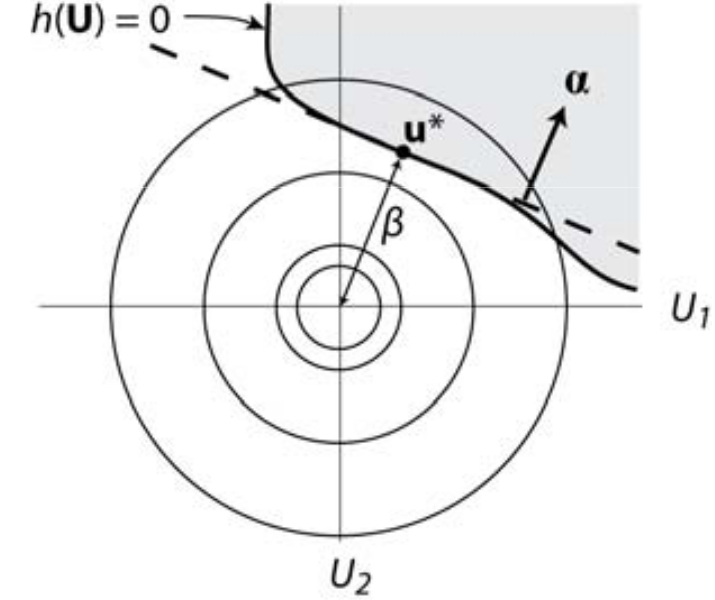
\includegraphics{FORM.jpg}}
\label{theory:form}\end{figure}


\subsection{Armijo Rule}
\label{theory:armijo-rule}
Denote a univariate function $\phi$ restricted to the direction
$\mathbf{p}_k$ as $\phi(\alpha)=f(\mathbf{x}_k+\alpha\mathbf{p}_k)$.
A step length $\alpha_k$ is said to satisfy the Wolfe conditions if the
following two inequalities hold:
\begin{gather}
\begin{split}i) f(\mathbf{x}_k+\alpha_k\mathbf{p}_k)\leq
   f(\mathbf{x}_k)+c_1\alpha_k\mathbf{p}_k^{\mathrm T}\nabla
   f(\mathbf{x}_k)\end{split}\notag\\\begin{split}\end{split}\notag
\end{gather}\begin{gather}
\begin{split}ii) \mathbf{p}_k^{\mathrm T}\nabla f(\mathbf{x}_k+\alpha_k\mathbf{p}_k)
    \geq c_2\mathbf{p}_k^{\mathrm T}\nabla f(\mathbf{x}_k)\end{split}\notag\\\begin{split}\end{split}\notag
\end{gather}
with $0<c_1<c_2<1$. (In examining condition (ii), recall that to ensure
that $\mathbf{p}_k$ is a descent direction, we have
$\mathbf{p}_k^{\mathrm T}\nabla f(\mathbf{x}_k) < 0$ .)

$c_1$ is usually chosen to be quite small while $c_2$ is much
larger; Nocedal gives example values of $c_1=10^{-4}$ and
$c_2=0.9$ for Newton or quasi-Newton methods and $c_2=0.1$ for the
nonlinear conjugate gradient method. Inequality i) is known as the Armijo rule
and ii) as the curvature condition; i) ensures that the step length
$\alpha_k$ decreases $f$ `sufficiently', and ii) ensures that the
slope has been reduced sufficiently.


\section{Cholesky decomposition}
\label{theory:cholesky-decomposition}
The Cholesky decomposition of a Hermitian positive-definite matrix A is a
decomposition of the form
\begin{gather}
\begin{split}\mathbf{A = L L}^{*}\end{split}\notag\\\begin{split}\end{split}\notag
\end{gather}
where L is a lower triangular matrix with positive diagonal entries, and L*
denotes the conjugate transpose of L. Every Hermitian positive-definite matrix
(and thus also every real-valued symmetric positive-definite matrix) has a
unique Cholesky decomposition.

If the matrix A is Hermitian and positive semi-definite, then it still has a
decomposition of the form A = LL* if the diagonal entries of L are allowed to
be zero.

When A has real entries, L has real entries as well.

The Cholesky decomposition is unique when A is positive definite; there is
only one lower triangular matrix L with strictly positive diagonal entries
such that A = LL*. However, the decomposition need not be unique when A is
positive semidefinite.

The converse holds trivially: if A can be written as LL* for some invertible
L, lower triangular or otherwise, then A is Hermitian and positive definite.


\section{Gauss base points and weight factors}
\label{theory:gauss-base-points-and-weight-factors}
using the algorithm given by Davis and Rabinowitz in `Methods of Numerical
Integration', page 365, Academic Press, 1975.


\chapter{Reliability Model}
\label{model:chap-model}\label{model::doc}\label{model:reliability-model}

\section{Inputparameter}
\label{model:module-pyre.model}\label{model:inputparameter}\index{pyre.model (module)}\index{AnalysisOptions (class in pyre.model)}

\begin{fulllineitems}
\phantomsection\label{model:pyre.model.AnalysisOptions}\pysigline{\strong{class }\code{pyre.model.}\bfcode{AnalysisOptions}}~\index{Ro\_method (pyre.model.AnalysisOptions attribute)}

\begin{fulllineitems}
\phantomsection\label{model:pyre.model.AnalysisOptions.Ro_method}\pysigline{\bfcode{Ro\_method}\strong{ = None}}
Method for computation of the modified Nataf correlation matrix
\begin{description}
\item[{Ro\_methods:}] \leavevmode\begin{itemize}
\item {} 
0: use of approximations from ADK's paper (no longer supported)

\item {} 
1: exact, solved numerically

\end{itemize}

\end{description}

\end{fulllineitems}

\index{block\_size (pyre.model.AnalysisOptions attribute)}

\begin{fulllineitems}
\phantomsection\label{model:pyre.model.AnalysisOptions.block_size}\pysigline{\bfcode{block\_size}\strong{ = None}}
Block size

Number of g-calls to be sent simultaneously

\end{fulllineitems}

\index{differentation\_modus (pyre.model.AnalysisOptions attribute)}

\begin{fulllineitems}
\phantomsection\label{model:pyre.model.AnalysisOptions.differentation_modus}\pysigline{\bfcode{differentation\_modus}\strong{ = None}}
Kind of differentiation
\begin{itemize}
\item {} 
`ddm': direct differentiation,

\item {} 
`ffd': forward finite difference

\end{itemize}

\end{fulllineitems}

\index{e1 (pyre.model.AnalysisOptions attribute)}

\begin{fulllineitems}
\phantomsection\label{model:pyre.model.AnalysisOptions.e1}\pysigline{\bfcode{e1}\strong{ = None}}
Tolerance on how close design point is to limit-state surface

\end{fulllineitems}

\index{e2 (pyre.model.AnalysisOptions attribute)}

\begin{fulllineitems}
\phantomsection\label{model:pyre.model.AnalysisOptions.e2}\pysigline{\bfcode{e2}\strong{ = None}}
Tolerance on how accurately the gradient points towards the origin

\end{fulllineitems}

\index{ffdpara (pyre.model.AnalysisOptions attribute)}

\begin{fulllineitems}
\phantomsection\label{model:pyre.model.AnalysisOptions.ffdpara}\pysigline{\bfcode{ffdpara}\strong{ = None}}
Parameter for computation

Parameter for computation of FFD estimates of gradients - Perturbation =
stdv/analysisopt.ffdpara
\begin{description}
\item[{Recommended values:}] \leavevmode\begin{itemize}
\item {} 
1000 for basic limit-state functions,

\item {} 
50 for FE-based limit-state functions

\end{itemize}

\end{description}

\end{fulllineitems}

\index{flag\_sens (pyre.model.AnalysisOptions attribute)}

\begin{fulllineitems}
\phantomsection\label{model:pyre.model.AnalysisOptions.flag_sens}\pysigline{\bfcode{flag\_sens}\strong{ = None}}
Flag for computation of sensitivities
\begin{description}
\item[{w.r.t. means, standard deviations, parameters and correlation coefficients}] \leavevmode\begin{itemize}
\item {} 
1: all sensitivities assessed,

\item {} 
0: no sensitivities assessment

\end{itemize}

\end{description}

\end{fulllineitems}

\index{i\_max (pyre.model.AnalysisOptions attribute)}

\begin{fulllineitems}
\phantomsection\label{model:pyre.model.AnalysisOptions.i_max}\pysigline{\bfcode{i\_max}\strong{ = None}}
Maximum number of iterations allowed in the search algorithm

\end{fulllineitems}

\index{multi\_proc (pyre.model.AnalysisOptions attribute)}

\begin{fulllineitems}
\phantomsection\label{model:pyre.model.AnalysisOptions.multi_proc}\pysigline{\bfcode{multi\_proc}\strong{ = None}}
Amount of g-calls
\begin{description}
\item[{1: block\_size g-calls sent simultaneously}] \leavevmode\begin{itemize}
\item {} 
gfunbasic.m is used and a vectorized version of gfundata.expression
is available. The number of g-calls sent simultaneously (block\_size)
depends on the memory available on the computer running FERUM.

\item {} 
gfunxxx.m user-specific g-function is used and able to handle
block\_size computations            sent simultaneously, on a cluster
of PCs or any other multiprocessor computer platform.

\end{itemize}

\end{description}

0: g-calls sent sequentially

\end{fulllineitems}

\index{print\_output (pyre.model.AnalysisOptions attribute)}

\begin{fulllineitems}
\phantomsection\label{model:pyre.model.AnalysisOptions.print_output}\pysigline{\bfcode{print\_output}\strong{ = None}}
Print comments during calculation
\begin{itemize}
\item {} 
True: FERUM interactive mode,

\item {} 
False: FERUM silent mode

\end{itemize}

\end{fulllineitems}

\index{step\_size (pyre.model.AnalysisOptions attribute)}

\begin{fulllineitems}
\phantomsection\label{model:pyre.model.AnalysisOptions.step_size}\pysigline{\bfcode{step\_size}\strong{ = None}}
Step size

0: step size by Armijo rule, otherwise: given value is the step size

\end{fulllineitems}

\index{transf\_type (pyre.model.AnalysisOptions attribute)}

\begin{fulllineitems}
\phantomsection\label{model:pyre.model.AnalysisOptions.transf_type}\pysigline{\bfcode{transf\_type}\strong{ = None}}
Type of joint distribution
\begin{description}
\item[{transf\_types:}] \leavevmode\begin{itemize}
\item {} 
1: jointly normal (no longer supported)

\item {} 
2: independent non-normal (no longer supported)

\item {} 
3: Nataf joint distribution (only available option)

\end{itemize}

\end{description}

\end{fulllineitems}


\end{fulllineitems}

\index{LimitState (class in pyre.model)}

\begin{fulllineitems}
\phantomsection\label{model:pyre.model.LimitState}\pysigline{\strong{class }\code{pyre.model.}\bfcode{LimitState}}~\index{evaluator (pyre.model.LimitState attribute)}

\begin{fulllineitems}
\phantomsection\label{model:pyre.model.LimitState.evaluator}\pysigline{\bfcode{evaluator}\strong{ = None}}
Type of limit-state function evaluator:
\begin{description}
\item[{`basic': the limit-state function is defined by means of an analytical}] \leavevmode
expression or a Matlab m-function, using
gfundata(lsf).expression. The function gfun.m calls gfunbasic.m,
which evaluates gfundata(lsf).expression.

\item[{`xxx':   the limit-state function evaluation requires a call to an}] \leavevmode
external code.  The function gfun.m calls gfunxxx.m, which
evaluates gfundata(lsf).expression where gext variable is a
result of the external code.

\end{description}

\end{fulllineitems}

\index{expression (pyre.model.LimitState attribute)}

\begin{fulllineitems}
\phantomsection\label{model:pyre.model.LimitState.expression}\pysigline{\bfcode{expression}\strong{ = None}}
Expression of the limit-state function

\end{fulllineitems}

\index{flag\_sens (pyre.model.LimitState attribute)}

\begin{fulllineitems}
\phantomsection\label{model:pyre.model.LimitState.flag_sens}\pysigline{\bfcode{flag\_sens}\strong{ = None}}
Flag for computation of sensitivities
\begin{description}
\item[{w.r.t. thetag parameters of the limit-state function}] \leavevmode\begin{itemize}
\item {} 
1: all sensitivities assessed,

\item {} 
0: no sensitivities assessment

\end{itemize}

\end{description}

\end{fulllineitems}


\end{fulllineitems}

\index{StochasticModel (class in pyre.model)}

\begin{fulllineitems}
\phantomsection\label{model:pyre.model.StochasticModel}\pysigline{\strong{class }\code{pyre.model.}\bfcode{StochasticModel}}
\end{fulllineitems}



\chapter{Calculations}
\label{calculations:chap-calculations}\label{calculations::doc}\label{calculations:calculations}

\section{Reliability}
\label{calculations:reliability}

\subsection{First-Order Reliability Method (FORM)}
\label{calculations:first-order-reliability-method-form}\label{calculations:module-pyre.form}\index{pyre.form (module)}\index{Form (class in pyre.form)}

\begin{fulllineitems}
\phantomsection\label{calculations:pyre.form.Form}\pysiglinewithargsret{\strong{class }\code{pyre.form.}\bfcode{Form}}{\emph{analysis\_options=None}, \emph{limit\_state=None}, \emph{stochastic\_model=None}}{}
\end{fulllineitems}

\phantomsection\label{calculations:module-pyre.limitstate}\index{pyre.limitstate (module)}\phantomsection\label{calculations:module-pyre.stepsize}\index{pyre.stepsize (module)}

\subsection{Second-Order Reliability Method (FORM)}
\label{calculations:second-order-reliability-method-form}

\section{Matrices Operators}
\label{calculations:matrices-operators}

\subsection{Cholesky decomposition}
\label{calculations:cholesky-decomposition}\label{calculations:module-pyre.cholesky}\index{pyre.cholesky (module)}

\subsection{Transformation}
\label{calculations:transformation}\label{calculations:module-pyre.transformation}\index{pyre.transformation (module)}

\section{Numerical Integration}
\label{calculations:module-pyre.quadrature}\label{calculations:numerical-integration}\index{pyre.quadrature (module)}\phantomsection\label{calculations:module-pyre.integration}\index{pyre.integration (module)}

\chapter{Probability distributions}
\label{distributions:chap-distributions}\label{distributions::doc}\label{distributions:probability-distributions}
PyRe provides a large suite of built-in probability distributions. For each distribution, it provides:
\begin{itemize}
\item {} 
A function that evaluates its marginal distribution.

\item {} 
A function that evaluates its probability density function.

\item {} 
A function that evaluates its cumulative distribution function.

\item {} 
A function that compute its jacobian.

\item {} 
A function that transform from from u to x space.

\item {} 
A function that transform from from x to u space.

\end{itemize}


\section{Normal distribution}
\label{distributions:normal-distribution}

\begin{fulllineitems}
\pysiglinewithargsret{\strong{class }\code{pyre.distributions.normal.}\bfcode{Normal}}{\emph{name}, \emph{mean}, \emph{stdv}, \emph{input\_type=None}, \emph{startpoint=None}}{}
Normal distribution
\begin{quote}\begin{description}
\item[{Attributes }] \leavevmode\begin{itemize}
\item {} 
name (str):         Name of the random variable

\item {} 
mean (float):       Mean

\item {} 
stdv (float):       Standard deviation

\item {} 
input\_type (any):   Change meaning of mean and stdv

\item {} 
startpoint (float): Start point for seach

\end{itemize}

\end{description}\end{quote}


\begin{fulllineitems}
\pysiglinewithargsret{\strong{classmethod }\code{Normal.}\bfcode{cdf}}{\emph{x}, \emph{mean=None}, \emph{stdv=None}, \emph{var\_3=None}, \emph{var\_4=None}}{}
cumulative distribution function

\end{fulllineitems}



\begin{fulllineitems}
\pysiglinewithargsret{\strong{classmethod }\code{Normal.}\bfcode{inv\_cdf}}{\emph{P}}{}
inverse cumulative distribution function

\end{fulllineitems}



\begin{fulllineitems}
\pysiglinewithargsret{\strong{classmethod }\code{Normal.}\bfcode{jacobian}}{\emph{u}, \emph{x}, \emph{marg}, \emph{J=None}}{}
Compute the Jacobian

\end{fulllineitems}



\begin{fulllineitems}
\pysiglinewithargsret{\strong{classmethod }\code{Normal.}\bfcode{pdf}}{\emph{x}, \emph{mean=None}, \emph{stdv=None}, \emph{var\_3=None}, \emph{var\_4=None}}{}
probability density function

\end{fulllineitems}



\begin{fulllineitems}
\pysiglinewithargsret{\code{Normal.}\bfcode{setMarginalDistribution}}{}{}
Compute the marginal distribution

\end{fulllineitems}



\begin{fulllineitems}
\pysiglinewithargsret{\strong{classmethod }\code{Normal.}\bfcode{u\_to\_x}}{\emph{u}, \emph{marg}, \emph{x=None}}{}
Transformation from u to x

\end{fulllineitems}



\begin{fulllineitems}
\pysiglinewithargsret{\strong{classmethod }\code{Normal.}\bfcode{x\_to\_u}}{\emph{x}, \emph{marg}, \emph{u=None}}{}
Transformation from x to u

\end{fulllineitems}


\end{fulllineitems}



\section{Lognormal distribution}
\label{distributions:lognormal-distribution}

\begin{fulllineitems}
\pysiglinewithargsret{\strong{class }\code{pyre.distributions.lognormal.}\bfcode{Lognormal}}{\emph{name}, \emph{mean}, \emph{stdv}, \emph{input\_type=None}, \emph{startpoint=None}}{}
Lognormal distribution
\begin{quote}\begin{description}
\item[{Arguments }] \leavevmode\begin{itemize}
\item {} 
name (str):         Name of the random variable

\item {} 
mean (float):       Mean or lamb

\item {} 
stdv (float):       Standard deviation or zeta

\item {} 
input\_type (any):   Change meaning of mean and stdv

\item {} 
startpoint (float): Start point for seach

\end{itemize}

\end{description}\end{quote}


\begin{fulllineitems}
\pysiglinewithargsret{\strong{classmethod }\code{Lognormal.}\bfcode{cdf}}{\emph{x}, \emph{lamb=None}, \emph{zeta=None}, \emph{var\_3=None}, \emph{var\_4=None}}{}
cumulative distribution function

\end{fulllineitems}



\begin{fulllineitems}
\pysiglinewithargsret{\strong{classmethod }\code{Lognormal.}\bfcode{jacobian}}{\emph{u}, \emph{x}, \emph{marg}, \emph{J=None}}{}
Compute the Jacobian

\end{fulllineitems}



\begin{fulllineitems}
\pysiglinewithargsret{\strong{classmethod }\code{Lognormal.}\bfcode{pdf}}{\emph{x}, \emph{lamb=None}, \emph{zeta=None}, \emph{var\_3=None}, \emph{var\_4=None}}{}
probability density function

\end{fulllineitems}



\begin{fulllineitems}
\pysiglinewithargsret{\code{Lognormal.}\bfcode{setMarginalDistribution}}{}{}
Compute the marginal distribution

\end{fulllineitems}



\begin{fulllineitems}
\pysiglinewithargsret{\strong{classmethod }\code{Lognormal.}\bfcode{u\_to\_x}}{\emph{u}, \emph{marg}, \emph{x=None}}{}
Transformation from u to x

\end{fulllineitems}



\begin{fulllineitems}
\pysiglinewithargsret{\strong{classmethod }\code{Lognormal.}\bfcode{x\_to\_u}}{\emph{x}, \emph{marg}, \emph{u=None}}{}
Transformation from x to u

\end{fulllineitems}


\end{fulllineitems}



\section{Gamma distribution}
\label{distributions:gamma-distribution}

\begin{fulllineitems}
\pysiglinewithargsret{\strong{class }\code{pyre.distributions.gamma.}\bfcode{Gamma}}{\emph{name}, \emph{mean}, \emph{stdv}, \emph{input\_type=None}, \emph{startpoint=None}}{}
Gamma distribution
\begin{quote}\begin{description}
\item[{Attributes }] \leavevmode\begin{itemize}
\item {} 
name (str):         Name of the random variable

\item {} 
mean (float):       Mean or lamb

\item {} 
stdv (float):       Standard deviation or k

\item {} 
input\_type (any):   Change meaning of mean and stdv

\item {} 
startpoint (float): Start point for seach

\end{itemize}

\end{description}\end{quote}


\begin{fulllineitems}
\pysiglinewithargsret{\strong{classmethod }\code{Gamma.}\bfcode{cdf}}{\emph{x}, \emph{lamb=None}, \emph{k=None}, \emph{var\_3=None}, \emph{var\_4=None}}{}
cumulative distribution function

\end{fulllineitems}



\begin{fulllineitems}
\pysiglinewithargsret{\strong{classmethod }\code{Gamma.}\bfcode{jacobian}}{\emph{u}, \emph{x}, \emph{marg}, \emph{J=None}}{}
Compute the Jacobian

\end{fulllineitems}



\begin{fulllineitems}
\pysiglinewithargsret{\strong{classmethod }\code{Gamma.}\bfcode{pdf}}{\emph{x}, \emph{lamb=None}, \emph{k=None}, \emph{var\_3=None}, \emph{var\_4=None}}{}
probability density function

\end{fulllineitems}



\begin{fulllineitems}
\pysiglinewithargsret{\code{Gamma.}\bfcode{setMarginalDistribution}}{}{}
Compute the marginal distribution

\end{fulllineitems}



\begin{fulllineitems}
\pysiglinewithargsret{\strong{classmethod }\code{Gamma.}\bfcode{u\_to\_x}}{\emph{u}, \emph{marg}, \emph{x=None}}{}
Transformation from u to x

\end{fulllineitems}



\begin{fulllineitems}
\pysiglinewithargsret{\strong{classmethod }\code{Gamma.}\bfcode{x\_to\_u}}{\emph{x}, \emph{marg}, \emph{u=None}}{}
Transformation from x to u

\end{fulllineitems}


\end{fulllineitems}



\section{Shifted exponential distribution}
\label{distributions:shifted-exponential-distribution}

\begin{fulllineitems}
\pysiglinewithargsret{\strong{class }\code{pyre.distributions.shiftedexponential.}\bfcode{ShiftedExponential}}{\emph{name}, \emph{mean}, \emph{stdv}, \emph{input\_type=None}, \emph{startpoint=None}}{}
Shifted exponential distribution
\begin{quote}\begin{description}
\item[{Attributes }] \leavevmode\begin{itemize}
\item {} 
name (str):         Name of the random variable

\item {} 
mean (float):       Mean or lamb

\item {} 
stdv (float):       Standard deviation or x\_zero

\item {} 
input\_type (any):   Change meaning of mean and stdv

\item {} 
startpoint (float): Start point for seach

\end{itemize}

\end{description}\end{quote}


\begin{fulllineitems}
\pysiglinewithargsret{\strong{classmethod }\code{ShiftedExponential.}\bfcode{cdf}}{\emph{x}, \emph{lamb=None}, \emph{x\_zero=None}, \emph{var\_3=None}, \emph{var\_4=None}}{}
cumulative distribution function

\end{fulllineitems}



\begin{fulllineitems}
\pysiglinewithargsret{\strong{classmethod }\code{ShiftedExponential.}\bfcode{jacobian}}{\emph{u}, \emph{x}, \emph{marg}, \emph{J=None}}{}
Compute the Jacobian

\end{fulllineitems}



\begin{fulllineitems}
\pysiglinewithargsret{\strong{classmethod }\code{ShiftedExponential.}\bfcode{pdf}}{\emph{x}, \emph{lamb=None}, \emph{x\_zero=None}, \emph{var\_3=None}, \emph{var\_4=None}}{}
probability density function

\end{fulllineitems}



\begin{fulllineitems}
\pysiglinewithargsret{\code{ShiftedExponential.}\bfcode{setMarginalDistribution}}{}{}
Compute the marginal distribution

\end{fulllineitems}



\begin{fulllineitems}
\pysiglinewithargsret{\strong{classmethod }\code{ShiftedExponential.}\bfcode{u\_to\_x}}{\emph{u}, \emph{marg}, \emph{x=None}}{}
Transformation from u to x

\end{fulllineitems}



\begin{fulllineitems}
\pysiglinewithargsret{\strong{classmethod }\code{ShiftedExponential.}\bfcode{x\_to\_u}}{\emph{x}, \emph{marg}, \emph{u=None}}{}
Transformation from x to u

\end{fulllineitems}


\end{fulllineitems}



\section{Shifted Rayleigh distribution}
\label{distributions:shifted-rayleigh-distribution}

\begin{fulllineitems}
\pysiglinewithargsret{\strong{class }\code{pyre.distributions.shiftedrayleigh.}\bfcode{ShiftedRayleigh}}{\emph{name}, \emph{mean}, \emph{stdv}, \emph{input\_type=None}, \emph{startpoint=None}}{}
Shifted Rayleigh distribution
\begin{quote}\begin{description}
\item[{Attributes }] \leavevmode\begin{itemize}
\item {} 
name (str):   Name of the random variable

\item {} 
mean (float): Mean or a

\item {} 
stdv (float): Standard deviation or x\_zero

\item {} 
input\_type (any): Change meaning of mean and stdv

\item {} 
startpoint (float): Start point for seach

\end{itemize}

\end{description}\end{quote}


\begin{fulllineitems}
\pysiglinewithargsret{\strong{classmethod }\code{ShiftedRayleigh.}\bfcode{cdf}}{\emph{x}, \emph{a=None}, \emph{x\_zero=None}, \emph{var\_3=None}, \emph{var\_4=None}}{}
cumulative distribution function

\end{fulllineitems}



\begin{fulllineitems}
\pysiglinewithargsret{\strong{classmethod }\code{ShiftedRayleigh.}\bfcode{jacobian}}{\emph{u}, \emph{x}, \emph{marg}, \emph{J=None}}{}
Compute the Jacobian

\end{fulllineitems}



\begin{fulllineitems}
\pysiglinewithargsret{\strong{classmethod }\code{ShiftedRayleigh.}\bfcode{pdf}}{\emph{x}, \emph{a=None}, \emph{x\_zero=None}, \emph{var\_3=None}, \emph{var\_4=None}}{}
probability density function

\end{fulllineitems}



\begin{fulllineitems}
\pysiglinewithargsret{\code{ShiftedRayleigh.}\bfcode{setMarginalDistribution}}{}{}
Compute the marginal distribution

\end{fulllineitems}



\begin{fulllineitems}
\pysiglinewithargsret{\strong{classmethod }\code{ShiftedRayleigh.}\bfcode{u\_to\_x}}{\emph{u}, \emph{marg}, \emph{x=None}}{}
Transformation from u to x

\end{fulllineitems}



\begin{fulllineitems}
\pysiglinewithargsret{\strong{classmethod }\code{ShiftedRayleigh.}\bfcode{x\_to\_u}}{\emph{x}, \emph{marg}, \emph{u=None}}{}
Transformation from x to u

\end{fulllineitems}


\end{fulllineitems}



\section{Uniform distribution}
\label{distributions:uniform-distribution}

\begin{fulllineitems}
\pysiglinewithargsret{\strong{class }\code{pyre.distributions.uniform.}\bfcode{Uniform}}{\emph{name}, \emph{mean}, \emph{stdv}, \emph{input\_type=None}, \emph{startpoint=None}}{}
Uniform distribution
\begin{quote}\begin{description}
\item[{Attributes }] \leavevmode\begin{itemize}
\item {} 
name (str):   Name of the random variable

\item {} 
mean (float): Mean or a

\item {} 
stdv (float): Standard deviation or b

\item {} 
input\_type (any): Change meaning of mean and stdv

\item {} 
startpoint (float): Start point for seach

\end{itemize}

\end{description}\end{quote}


\begin{fulllineitems}
\pysiglinewithargsret{\strong{classmethod }\code{Uniform.}\bfcode{cdf}}{\emph{x}, \emph{a=None}, \emph{b=None}, \emph{var\_3=None}, \emph{var\_4=None}}{}
cumulative distribution function

\end{fulllineitems}



\begin{fulllineitems}
\pysiglinewithargsret{\strong{classmethod }\code{Uniform.}\bfcode{jacobian}}{\emph{u}, \emph{x}, \emph{marg}, \emph{J=None}}{}
Compute the Jacobian

\end{fulllineitems}



\begin{fulllineitems}
\pysiglinewithargsret{\strong{classmethod }\code{Uniform.}\bfcode{pdf}}{\emph{x}, \emph{a=None}, \emph{b=None}, \emph{var\_3=None}, \emph{var\_4=None}}{}
probability density function

\end{fulllineitems}



\begin{fulllineitems}
\pysiglinewithargsret{\code{Uniform.}\bfcode{setMarginalDistribution}}{}{}
Compute the marginal distribution

\end{fulllineitems}



\begin{fulllineitems}
\pysiglinewithargsret{\strong{classmethod }\code{Uniform.}\bfcode{u\_to\_x}}{\emph{u}, \emph{marg}, \emph{x=None}}{}
Transformation from u to x

\end{fulllineitems}



\begin{fulllineitems}
\pysiglinewithargsret{\strong{classmethod }\code{Uniform.}\bfcode{x\_to\_u}}{\emph{x}, \emph{marg}, \emph{u=None}}{}
Transformation from x to u

\end{fulllineitems}


\end{fulllineitems}



\section{Beta distribution}
\label{distributions:beta-distribution}

\begin{fulllineitems}
\pysiglinewithargsret{\strong{class }\code{pyre.distributions.beta.}\bfcode{Beta}}{\emph{name}, \emph{mean}, \emph{stdv}, \emph{a=0}, \emph{b=1}, \emph{input\_type=None}, \emph{startpoint=None}}{}
Beta distribution
\begin{quote}\begin{description}
\item[{Attributes }] \leavevmode\begin{itemize}
\item {} 
name (str):   Name of the random variable

\item {} 
mean (float): Mean or q

\item {} 
stdv (float): Standard deviation or r

\item {} 
a (float):    Lower boundary

\item {} 
b (float):    Uper boundary

\item {} 
input\_type (any): Change meaning of mean and stdv

\item {} 
startpoint (float): Start point for seach

\end{itemize}

\end{description}\end{quote}


\begin{fulllineitems}
\pysiglinewithargsret{\strong{classmethod }\code{Beta.}\bfcode{cdf}}{\emph{x}, \emph{q=None}, \emph{r=None}, \emph{a=None}, \emph{b=None}}{}
cumulative distribution function

\end{fulllineitems}



\begin{fulllineitems}
\pysiglinewithargsret{\strong{classmethod }\code{Beta.}\bfcode{jacobian}}{\emph{u}, \emph{x}, \emph{marg}, \emph{J=None}}{}
Compute the Jacobian

\end{fulllineitems}



\begin{fulllineitems}
\pysiglinewithargsret{\strong{classmethod }\code{Beta.}\bfcode{pdf}}{\emph{x}, \emph{q=None}, \emph{r=None}, \emph{a=None}, \emph{b=None}}{}
probability density function

\end{fulllineitems}



\begin{fulllineitems}
\pysiglinewithargsret{\code{Beta.}\bfcode{setMarginalDistribution}}{}{}
Compute the marginal distribution

\end{fulllineitems}



\begin{fulllineitems}
\pysiglinewithargsret{\strong{classmethod }\code{Beta.}\bfcode{u\_to\_x}}{\emph{u}, \emph{marg}, \emph{x=None}}{}
Transformation from u to x

\end{fulllineitems}



\begin{fulllineitems}
\pysiglinewithargsret{\strong{classmethod }\code{Beta.}\bfcode{x\_to\_u}}{\emph{x}, \emph{marg}, \emph{u=None}}{}
Transformation from x to u

\end{fulllineitems}


\end{fulllineitems}



\section{Chi square distribution}
\label{distributions:chi-square-distribution}

\begin{fulllineitems}
\pysiglinewithargsret{\strong{class }\code{pyre.distributions.chisquare.}\bfcode{ChiSquare}}{\emph{name}, \emph{mean}, \emph{stdv=None}, \emph{input\_type=None}, \emph{startpoint=None}}{}
Chi-Square distribution
\begin{quote}\begin{description}
\item[{Attributes }] \leavevmode\begin{itemize}
\item {} 
name (str):   Name of the random variable

\item {} 
mean (float): Mean or nu

\item {} 
stdv (float): Standard deviation

\item {} 
input\_type (any): Change meaning of mean and stdv

\item {} 
startpoint (float): Start point for seach

\end{itemize}

\end{description}\end{quote}


\begin{fulllineitems}
\pysiglinewithargsret{\strong{classmethod }\code{ChiSquare.}\bfcode{cdf}}{\emph{x}, \emph{nu=None}, \emph{var\_2=None}, \emph{var\_3=None}, \emph{var\_4=None}}{}
cumulative distribution function

\end{fulllineitems}



\begin{fulllineitems}
\pysiglinewithargsret{\strong{classmethod }\code{ChiSquare.}\bfcode{jacobian}}{\emph{u}, \emph{x}, \emph{marg}, \emph{J=None}}{}
Compute the Jacobian

\end{fulllineitems}



\begin{fulllineitems}
\pysiglinewithargsret{\strong{classmethod }\code{ChiSquare.}\bfcode{pdf}}{\emph{x}, \emph{nu=None}, \emph{var\_2=None}, \emph{var\_3=None}, \emph{var\_4=None}}{}
probability density function

\end{fulllineitems}



\begin{fulllineitems}
\pysiglinewithargsret{\code{ChiSquare.}\bfcode{setMarginalDistribution}}{}{}
Compute the marginal distribution

\end{fulllineitems}



\begin{fulllineitems}
\pysiglinewithargsret{\strong{classmethod }\code{ChiSquare.}\bfcode{u\_to\_x}}{\emph{u}, \emph{marg}, \emph{x=None}}{}
Transformation from u to x

\end{fulllineitems}



\begin{fulllineitems}
\pysiglinewithargsret{\strong{classmethod }\code{ChiSquare.}\bfcode{x\_to\_u}}{\emph{x}, \emph{marg}, \emph{u=None}}{}
Transformation from x to u

\end{fulllineitems}


\end{fulllineitems}



\section{Type I largest value distribution}
\label{distributions:type-i-largest-value-distribution}

\begin{fulllineitems}
\pysiglinewithargsret{\strong{class }\code{pyre.distributions.typeilargestvalue.}\bfcode{TypeIlargestValue}}{\emph{name}, \emph{mean}, \emph{stdv}, \emph{input\_type=None}, \emph{startpoint=None}}{}
Type I largest value distribution
\begin{quote}\begin{description}
\item[{Attributes }] \leavevmode\begin{itemize}
\item {} 
name (str):   Name of the random variable

\item {} 
mean (float): Mean or u\_n

\item {} 
stdv (float): Standard deviation or a\_n

\item {} 
input\_type (any): Change meaning of mean and stdv

\item {} 
startpoint (float): Start point for seach

\end{itemize}

\end{description}\end{quote}


\begin{fulllineitems}
\pysiglinewithargsret{\strong{classmethod }\code{TypeIlargestValue.}\bfcode{cdf}}{\emph{x}, \emph{u\_n=None}, \emph{a\_n=None}, \emph{var\_3=None}, \emph{var\_4=None}}{}
cumulative distribution function

\end{fulllineitems}



\begin{fulllineitems}
\pysiglinewithargsret{\strong{classmethod }\code{TypeIlargestValue.}\bfcode{jacobian}}{\emph{u}, \emph{x}, \emph{marg}, \emph{J=None}}{}
Compute the Jacobian

\end{fulllineitems}



\begin{fulllineitems}
\pysiglinewithargsret{\strong{classmethod }\code{TypeIlargestValue.}\bfcode{pdf}}{\emph{x}, \emph{u\_n=None}, \emph{a\_n=None}, \emph{var\_3=None}, \emph{var\_4=None}}{}
probability density function

\end{fulllineitems}



\begin{fulllineitems}
\pysiglinewithargsret{\code{TypeIlargestValue.}\bfcode{setMarginalDistribution}}{}{}
Compute the marginal distribution

\end{fulllineitems}



\begin{fulllineitems}
\pysiglinewithargsret{\strong{classmethod }\code{TypeIlargestValue.}\bfcode{u\_to\_x}}{\emph{u}, \emph{marg}, \emph{x=None}}{}
Transformation from u to x

\end{fulllineitems}



\begin{fulllineitems}
\pysiglinewithargsret{\strong{classmethod }\code{TypeIlargestValue.}\bfcode{x\_to\_u}}{\emph{x}, \emph{marg}, \emph{u=None}}{}
Transformation from x to u

\end{fulllineitems}


\end{fulllineitems}



\section{Type I smallest value distribution}
\label{distributions:type-i-smallest-value-distribution}

\begin{fulllineitems}
\pysiglinewithargsret{\strong{class }\code{pyre.distributions.typeismallestvalue.}\bfcode{TypeIsmallestValue}}{\emph{name}, \emph{mean}, \emph{stdv}, \emph{input\_type=None}, \emph{startpoint=None}}{}
Type I smallest value distribution
\begin{quote}\begin{description}
\item[{Attributes }] \leavevmode\begin{itemize}
\item {} 
name (str):   Name of the random variable

\item {} 
mean (float): Mean or u\_1

\item {} 
stdv (float): Standard deviation or a\_1

\item {} 
input\_type (any): Change meaning of mean and stdv

\item {} 
startpoint (float): Start point for seach

\end{itemize}

\end{description}\end{quote}


\begin{fulllineitems}
\pysiglinewithargsret{\strong{classmethod }\code{TypeIsmallestValue.}\bfcode{cdf}}{\emph{x}, \emph{u\_1=None}, \emph{a\_1=None}, \emph{var\_3=None}, \emph{var\_4=None}}{}
cumulative distribution function

\end{fulllineitems}



\begin{fulllineitems}
\pysiglinewithargsret{\strong{classmethod }\code{TypeIsmallestValue.}\bfcode{jacobian}}{\emph{u}, \emph{x}, \emph{marg}, \emph{J=None}}{}
Compute the Jacobian

\end{fulllineitems}



\begin{fulllineitems}
\pysiglinewithargsret{\strong{classmethod }\code{TypeIsmallestValue.}\bfcode{pdf}}{\emph{x}, \emph{u\_1=None}, \emph{a\_1=None}, \emph{var\_3=None}, \emph{var\_4=None}}{}
probability density function

\end{fulllineitems}



\begin{fulllineitems}
\pysiglinewithargsret{\code{TypeIsmallestValue.}\bfcode{setMarginalDistribution}}{}{}
Compute the marginal distribution

\end{fulllineitems}



\begin{fulllineitems}
\pysiglinewithargsret{\strong{classmethod }\code{TypeIsmallestValue.}\bfcode{u\_to\_x}}{\emph{u}, \emph{marg}, \emph{x=None}}{}
Transformation from u to x

\end{fulllineitems}



\begin{fulllineitems}
\pysiglinewithargsret{\strong{classmethod }\code{TypeIsmallestValue.}\bfcode{x\_to\_u}}{\emph{x}, \emph{marg}, \emph{u=None}}{}
Transformation from x to u

\end{fulllineitems}


\end{fulllineitems}



\section{Type II largest value distribution}
\label{distributions:type-ii-largest-value-distribution}

\begin{fulllineitems}
\pysiglinewithargsret{\strong{class }\code{pyre.distributions.typeiilargestvalue.}\bfcode{TypeIIlargestValue}}{\emph{name}, \emph{mean}, \emph{stdv}, \emph{input\_type=None}, \emph{startpoint=None}}{}
Type II largest value distribution
\begin{quote}\begin{description}
\item[{Attributes }] \leavevmode\begin{itemize}
\item {} 
name (str):   Name of the random variable

\item {} 
mean (float): Mean or u\_n

\item {} 
stdv (float): Standard deviation or k

\item {} 
input\_type (any): Change meaning of mean and stdv

\item {} 
startpoint (float): Start point for seach

\end{itemize}

\end{description}\end{quote}


\begin{fulllineitems}
\pysiglinewithargsret{\strong{classmethod }\code{TypeIIlargestValue.}\bfcode{cdf}}{\emph{x}, \emph{u\_n=None}, \emph{k=None}, \emph{var\_3=None}, \emph{var\_4=None}}{}
cumulative distribution function

\end{fulllineitems}



\begin{fulllineitems}
\pysiglinewithargsret{\strong{classmethod }\code{TypeIIlargestValue.}\bfcode{jacobian}}{\emph{u}, \emph{x}, \emph{marg}, \emph{J=None}}{}
Compute the Jacobian

\end{fulllineitems}



\begin{fulllineitems}
\pysiglinewithargsret{\strong{classmethod }\code{TypeIIlargestValue.}\bfcode{pdf}}{\emph{x}, \emph{u\_n=None}, \emph{k=None}, \emph{var\_3=None}, \emph{var\_4=None}}{}
probability density function

\end{fulllineitems}



\begin{fulllineitems}
\pysiglinewithargsret{\code{TypeIIlargestValue.}\bfcode{setMarginalDistribution}}{}{}
Compute the marginal distribution

\end{fulllineitems}



\begin{fulllineitems}
\pysiglinewithargsret{\strong{classmethod }\code{TypeIIlargestValue.}\bfcode{u\_to\_x}}{\emph{u}, \emph{marg}, \emph{x=None}}{}
Transformation from u to x

\end{fulllineitems}



\begin{fulllineitems}
\pysiglinewithargsret{\strong{classmethod }\code{TypeIIlargestValue.}\bfcode{x\_to\_u}}{\emph{x}, \emph{marg}, \emph{u=None}}{}
Transformation from x to u

\end{fulllineitems}


\end{fulllineitems}



\section{Type III smallest value distribution}
\label{distributions:type-iii-smallest-value-distribution}

\begin{fulllineitems}
\pysiglinewithargsret{\strong{class }\code{pyre.distributions.typeiiismallestvalue.}\bfcode{TypeIIIsmallestValue}}{\emph{name}, \emph{mean}, \emph{stdv}, \emph{epsilon=0}, \emph{input\_type=None}, \emph{startpoint=None}}{}
Type III smallest value distribution
\begin{quote}\begin{description}
\item[{Attributes }] \leavevmode\begin{itemize}
\item {} 
name (str):   Name of the random variable

\item {} 
mean (float): Mean or u\_1

\item {} 
stdv (float): Standard deviation or k

\item {} 
epsilon (float): Epsilon

\item {} 
input\_type (any): Change meaning of mean and stdv

\item {} 
startpoint (float): Start point for seach

\end{itemize}

\end{description}\end{quote}


\begin{fulllineitems}
\pysiglinewithargsret{\strong{classmethod }\code{TypeIIIsmallestValue.}\bfcode{cdf}}{\emph{x}, \emph{u\_1=None}, \emph{k=None}, \emph{epsilon=None}, \emph{var\_4=None}}{}
cumulative distribution function

\end{fulllineitems}



\begin{fulllineitems}
\pysiglinewithargsret{\strong{classmethod }\code{TypeIIIsmallestValue.}\bfcode{jacobian}}{\emph{u}, \emph{x}, \emph{marg}, \emph{J=None}}{}
Compute the Jacobian

\end{fulllineitems}



\begin{fulllineitems}
\pysiglinewithargsret{\strong{classmethod }\code{TypeIIIsmallestValue.}\bfcode{pdf}}{\emph{x}, \emph{u\_1=None}, \emph{k=None}, \emph{epsilon=None}, \emph{var\_4=None}}{}
probability density function

\end{fulllineitems}



\begin{fulllineitems}
\pysiglinewithargsret{\code{TypeIIIsmallestValue.}\bfcode{setMarginalDistribution}}{}{}
Compute the marginal distribution

\end{fulllineitems}



\begin{fulllineitems}
\pysiglinewithargsret{\strong{classmethod }\code{TypeIIIsmallestValue.}\bfcode{u\_to\_x}}{\emph{u}, \emph{marg}, \emph{x=None}}{}
Transformation from u to x

\end{fulllineitems}



\begin{fulllineitems}
\pysiglinewithargsret{\strong{classmethod }\code{TypeIIIsmallestValue.}\bfcode{x\_to\_u}}{\emph{x}, \emph{marg}, \emph{u=None}}{}
Transformation from x to u

\end{fulllineitems}


\end{fulllineitems}



\section{Gumbel distribution}
\label{distributions:gumbel-distribution}

\begin{fulllineitems}
\pysiglinewithargsret{\strong{class }\code{pyre.distributions.gumbel.}\bfcode{Gumbel}}{\emph{name}, \emph{mean}, \emph{stdv}, \emph{input\_type=None}, \emph{startpoint=None}}{}
Gumbel distribution
\begin{quote}\begin{description}
\item[{Attributes }] \leavevmode\begin{itemize}
\item {} 
name (str):   Name of the random variable

\item {} 
mean (float): Mean or u\_n

\item {} 
stdv (float): Standard deviation or a\_n

\item {} 
input\_type (any): Change meaning of mean and stdv

\item {} 
startpoint (float): Start point for seach

\end{itemize}

\end{description}\end{quote}


\begin{fulllineitems}
\pysiglinewithargsret{\strong{classmethod }\code{Gumbel.}\bfcode{cdf}}{\emph{x}, \emph{u\_n=None}, \emph{a\_n=None}, \emph{var\_3=None}, \emph{var\_4=None}}{}
cumulative distribution function

\end{fulllineitems}



\begin{fulllineitems}
\pysiglinewithargsret{\strong{classmethod }\code{Gumbel.}\bfcode{jacobian}}{\emph{u}, \emph{x}, \emph{marg}, \emph{J=None}}{}
Compute the Jacobian

\end{fulllineitems}



\begin{fulllineitems}
\pysiglinewithargsret{\strong{classmethod }\code{Gumbel.}\bfcode{pdf}}{\emph{x}, \emph{u\_n=None}, \emph{a\_n=None}, \emph{var\_3=None}, \emph{var\_4=None}}{}
probability density function

\end{fulllineitems}



\begin{fulllineitems}
\pysiglinewithargsret{\code{Gumbel.}\bfcode{setMarginalDistribution}}{}{}
Compute the marginal distribution

\end{fulllineitems}



\begin{fulllineitems}
\pysiglinewithargsret{\strong{classmethod }\code{Gumbel.}\bfcode{u\_to\_x}}{\emph{u}, \emph{marg}, \emph{x=None}}{}
Transformation from u to x

\end{fulllineitems}



\begin{fulllineitems}
\pysiglinewithargsret{\strong{classmethod }\code{Gumbel.}\bfcode{x\_to\_u}}{\emph{x}, \emph{marg}, \emph{u=None}}{}
Transformation from x to u

\end{fulllineitems}


\end{fulllineitems}



\section{Weibull distribution}
\label{distributions:weibull-distribution}

\begin{fulllineitems}
\pysiglinewithargsret{\strong{class }\code{pyre.distributions.weibull.}\bfcode{Weibull}}{\emph{name}, \emph{mean}, \emph{stdv}, \emph{epsilon=0}, \emph{input\_type=None}, \emph{startpoint=None}}{}
Weibull distribution
\begin{quote}\begin{description}
\item[{Attributes }] \leavevmode\begin{itemize}
\item {} 
name (str):   Name of the random variable

\item {} 
mean (float): Mean or u\_1

\item {} 
stdv (float): Standard deviation or k

\item {} 
epsilon (float): Epsilon

\item {} 
input\_type (any): Change meaning of mean and stdv

\item {} 
startpoint (float): Start point for seach

\end{itemize}

\end{description}\end{quote}


\begin{fulllineitems}
\pysiglinewithargsret{\strong{classmethod }\code{Weibull.}\bfcode{cdf}}{\emph{x}, \emph{u\_1=None}, \emph{k=None}, \emph{epsilon=None}, \emph{var\_4=None}}{}
cumulative distribution function

\end{fulllineitems}



\begin{fulllineitems}
\pysiglinewithargsret{\strong{classmethod }\code{Weibull.}\bfcode{jacobian}}{\emph{u}, \emph{x}, \emph{marg}, \emph{J=None}}{}
Compute the Jacobian

\end{fulllineitems}



\begin{fulllineitems}
\pysiglinewithargsret{\strong{classmethod }\code{Weibull.}\bfcode{pdf}}{\emph{x}, \emph{u\_1=None}, \emph{k=None}, \emph{epsilon=None}, \emph{var\_4=None}}{}
probability density function

\end{fulllineitems}



\begin{fulllineitems}
\pysiglinewithargsret{\code{Weibull.}\bfcode{setMarginalDistribution}}{}{}
Compute the marginal distribution

\end{fulllineitems}



\begin{fulllineitems}
\pysiglinewithargsret{\strong{classmethod }\code{Weibull.}\bfcode{u\_to\_x}}{\emph{u}, \emph{marg}, \emph{x=None}}{}
Transformation from u to x

\end{fulllineitems}



\begin{fulllineitems}
\pysiglinewithargsret{\strong{classmethod }\code{Weibull.}\bfcode{x\_to\_u}}{\emph{x}, \emph{marg}, \emph{u=None}}{}
Transformation from x to u

\end{fulllineitems}


\end{fulllineitems}



\chapter{List of References}
\label{references:list-of-references}\label{references::doc}

\chapter{Indices and tables}
\label{index:indices-and-tables}\begin{itemize}
\item {} 
\emph{genindex}

\item {} 
\emph{modindex}

\item {} 
\emph{search}

\end{itemize}

\begin{thebibliography}{DerKiureghian2006}
\bibitem[Bourinet2009]{Bourinet2009}{\phantomsection\label{references:bourinet2009} 
J.-M. Bourinet, C. Mattrand, and V Dubourg. A review of recent features and improvements added to FERUM software. In Proc. of the 10th International Conference on Structural Safety and Reliability (ICOSSAR’09), Osaka, Japan, 2009.
}
\bibitem[Bourinet2010]{Bourinet2010}{\phantomsection\label{references:bourinet2010} 
J.-M. Bourinet. FERUM 4.1 User’s Guide, 2010.
}
\bibitem[DerKiureghian2006]{DerKiureghian2006}{\phantomsection\label{references:derkiureghian2006} \begin{enumerate}
\item {} 
Der Kiureghian, T. Haukaas, and K. Fujimura. Structural reliability software at the University of California, Berkeley. Structural Safety, 28(1-2):44–67, 2006.

\end{enumerate}
}
\bibitem[Hackl2013]{Hackl2013}{\phantomsection\label{references:hackl2013} \begin{enumerate}
\setcounter{enumi}{9}
\item {} 
Hackl. Risk based decision framework for the optimal management of aging reinforced concrete structures. Master’s thesis, Norwegian University of Science and Technolog, Trondheim, Norway, 2013. (in work)

\end{enumerate}
}
\bibitem[Langtangen2009]{Langtangen2009}{\phantomsection\label{references:langtangen2009} 
Hans Petter Langtangen. Python Scripting for Computational Science. Springer-Verlag, 2009.
}
\bibitem[Lutz2007]{Lutz2007}{\phantomsection\label{references:lutz2007} \begin{enumerate}
\setcounter{enumi}{12}
\item {} 
Lutz. Learning Python. O’Reilly, 2007.

\end{enumerate}
}
\bibitem[Melchers1999]{Melchers1999}{\phantomsection\label{references:melchers1999} 
R.D. Melchers. structural reliability analysis and prediction Ellishorwood limited, Manchester, 1999.
}
\end{thebibliography}


\renewcommand{\indexname}{Python Module Index}
\begin{theindex}
\def\bigletter#1{{\Large\sffamily#1}\nopagebreak\vspace{1mm}}
\bigletter{p}
\item {\texttt{pyre.cholesky}}, \pageref{calculations:module-pyre.cholesky}
\item {\texttt{pyre.form}}, \pageref{calculations:module-pyre.form}
\item {\texttt{pyre.integration}}, \pageref{calculations:module-pyre.integration}
\item {\texttt{pyre.limitstate}}, \pageref{calculations:module-pyre.limitstate}
\item {\texttt{pyre.model}}, \pageref{model:module-pyre.model}
\item {\texttt{pyre.quadrature}}, \pageref{calculations:module-pyre.quadrature}
\item {\texttt{pyre.stepsize}}, \pageref{calculations:module-pyre.stepsize}
\item {\texttt{pyre.transformation}}, \pageref{calculations:module-pyre.transformation}
\end{theindex}

\renewcommand{\indexname}{Index}
\printindex
\end{document}
